\documentclass[Bachelorarbeit.tex]{subfiles}
\begin{document}

\graphicspath{{./figures/hypothesis/}}	%specifying the folder for the figures

\chapter{Hypothesis}
\label{ch:hypothesis}

In this chapter the question of the importance of fully-connectedness for reaching the equilibrium is raised where the question is whether it is really necessary to have a fully-connected network to reach equilibrium or not. We challenge this and claim that a much lower connectivity but a very special one is required and present a definition for it in a hypothesis which states that if a network satisfies the postulated properties of the hypothesis then using this network in the simulation will result in approaching the same equilibrium as found in fully-connected networks.

\section{Definition}

\begin{equation}
\begin{split}
\textit{fully-connectedness equilibrium} \iff \\
\forall \: \textit{agent-pairs} \: (a_{1},a_{n}) \: \exists \:  \textit{path} \: P \: \{a_{1}, a_{2}, ... , a_{n-1}, a_{n}\} \: | \: h(a_{i}) < h(a_{i+1})
\end{split}
\end{equation}

\newtheorem{conj}{Conjecture}

\begin{conj}
If and only if for all agents exists a path between two agents in which each visited agent has a larger optimism factor than the previous one then the same equilibrium as in fully-connectedness will be reached.
\end{conj}

The most minimal configuration of agents which satisfies this hypothesis is a graph of agents where each agent is connected to the agent with the next higher optimism-factor. This is the same as the Ascending-Connected topology - see appendix \ref{app:topologies} - which is the major network of interest in this thesis (besides the fully-connected one) as it is the most minimal topology which satisfies the hypothesis.

\section{Motivation}
The motivation behind the hypothesis is the fact that according to the double-auction definition - see chapter \ref{ch:theory} - for a match to happen the buyer-price must be larger or equal to the seller-price. This can only be the case when the buyer has a higher optimism-factor than the seller due the way agents place their prices - see chapter \ref{ch:leverageCycle}.

\subsection{Proof}
The proofs are given for the Asset/Cash market only because the equations of the Loan/Cash market work exactly the same way where only the absolute numbers are different. The Asset/Bond market is the same too as the limit-price is just the ratio of the limit-prices of asset and bond thus resulting in the same linear ordering of the limit-prices.

\paragraph{Visual proof}
In figure \ref{fig:MATCHING_BUYER_SELLER_RANGES} the price-ranges of both a seller and buyer are given where h(s) and h(b) denote the optimism-factors of the seller and buyer respectively. The seller places its offerings in the price-range of [h(s)..pU] as it wants to sell the good above the expected price to make a profit. The buyer places its offerings in the price-range of [pD..h(b)] as it wants to buy the goods below the expected price to make a profit. The resulting matching-range on which the prices can meet - again buyer-price $\geq$ seller-price - is marked by the red rectangle. It is easy to see that a match with these mechanics can occur only if the optimism-factor of the buyer h(b) is strictly higher than the one of the seller h(s).

\begin{figure}[H]
	\centering
  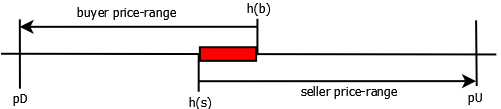
\includegraphics[width=1.0\textwidth, angle=0]{MATCHING_BUYER_SELLER_RANGES.png}
  	\caption{Matching of buyers and sellers price-ranges. The red rectangle marks the matching-range.}
	\label{fig:MATCHING_BUYER_SELLER_RANGES}
\end{figure}

\paragraph{Formal proof}
TODO

\section{Predictions}
The following topologies found in appendix \ref{app:topologies} satisfy the definition of the hypothesis:
 
\begin{itemize}
\item Fully-Connected
\item Half-Fully connected
\item Ascending-Connected
\item Ascending-Connected with all kind of short-cuts
\item Erdos-Renyi and Watts-Strogatz with the correct parametrization by pure chance.
\end{itemize}

It is expected that according to the hypothesis all of these topologies will reach the equilibrium found in fully-connectedness. All other topologies do not satisfy the hypothesis and are expected to clearly fail reaching the equilibrium of the Fully-Connected topology.

\medskip

See chapter \ref{ch:results} and \ref{ch:interpretation} whether the results reflect the hypothesis or not. 

\end{document}